\documentclass[11pt,a4paper]{article}
\usepackage[margin=2.2cm]{geometry}
\usepackage{graphicx,booktabs,hyperref,xcolor,float}
\hypersetup{colorlinks=true,linkcolor=blue!60!black,urlcolor=blue!60!black}
\title{Autonomous Ops Analytics Report}
\author{LLM-Orchestrated Pipeline (Python execution engine)}
\date{2026-09-10}
\begin{document}
\maketitle
Run ID: \texttt{sample\_run} \\
\section{Executive Summary}
Automated analysis of 200 rows x 6 columns produced 4 key finding(s). Strongest linear association is temperature\_rollmean3 vs temperature\_lag1 (|r|=0.863).
\section{Dataset Profile}
Rows: 200, Columns: 6. Timestamp: timestamp.\\
\begin{itemize}
\item \texttt{timestamp} (str) --- missing 0.0\% 
\item \texttt{temperature} (float64) --- missing 0.5\% 
\item \texttt{pressure} (float64) --- missing 0.0\% 
\item \texttt{vibration} (float64) --- missing 0.0\% 
\item \texttt{status} (str) --- missing 0.5\% 
\item \texttt{fault} (int64) --- missing 0.0\% 
\end{itemize}
\section{Analysis Plan (Stage-1)}
\begin{itemize}
\item cleaning: ["drop\_duplicates", "median\_mode\_fill"] 
\item analyses: ["correlation", "anomaly\_detection", "forecasting"] 
\item feature\_engineering: ["time\_features", "lags", "rolling\_stats"] 
\item visualizations: ["histograms", "time\_series", "forecast\_plot"] 
\item supervised: "random\_forest\_classifier" target=fault 
\end{itemize}
\section{Computed Results}
\subsection{Correlation}
\begin{verbatim}
{
  "status": "ok",
  "columns": [
    "temperature",
    "pressure",
    "vibration",
    "fault",
    "hour",
    "dayofweek",
    "month",
    "temperature_lag1",
    "pressure_lag1",
    "vibration_lag1",
    "temperature_rollmean3",
    "pressure_rollmean3",
    "vibration_rollmean3"
  ],
  "top_pairs": [
    {
      "a": "temperature_rollmean3",
      "b": "temperature_lag1",
      "abs_corr": 0.863
    },
    {
      "a": "temperature_lag1",
      "b": "temperature_rollmean3",
      "abs_corr": 0.863
    },
    {
      "a": "temperature",
      "b": "temperature_rollmean3",
      "abs_corr": 0.839
    },
    {
      "a": "temperature_rollmean3",
      "b": "temperature",
      "abs_corr": 0.839
    },
    {
      "a": "pressure_lag1",
      "b": "pressure_rollmean3",
      "abs_corr": 0.714
    },
    {
      "a": "pressure_rollmean3",
      "b": "pressure_lag1",
      "abs_corr": 0.714
    },
    {
      "a": "temperature_rollmean3",
      "b": "pressure_rollmean3",
      "abs_corr": 0.668
    },
    {
      "a": "pressure_rollmean3",
      "b": "temperature_rollmean3",
      "abs_corr": 0.668
    },
    {
      "a": "pressure_rollmean3",
      "b": "pressure",
      "abs_corr": 0.665
    },
    {
      "a": "pressure",
      "b": "pressure_rollmean3",
      "abs_corr": 0.665
    }
  ]
}
\end{verbatim}
\subsection{Clustering}
\begin{verbatim}
{}
\end{verbatim}
\subsection{Anomaly}
\begin{verbatim}
{
  "status": "ok",
  "method": "IsolationForest",
  "n_anomalies": 10,
  "anomaly_pct": 5.0
}
\end{verbatim}
\subsection{Forecast}
\begin{verbatim}
{
  "status": "ok",
  "method": "naive-last-value-backtest",
  "target": "temperature",
  "mae": 1.9407,
  "rmse": 2.2605,
  "n_train": 160,
  "n_test": 40
}
\end{verbatim}
\subsection{Supervised}
\begin{verbatim}
{
  "status": "ok",
  "task": "classification",
  "method": "random_forest_classifier",
  "accuracy": 1.0,
  "f1_macro": 1.0,
  "saved_pipeline": "models/supervised_pipeline.joblib"
}
\end{verbatim}
\section{Key Findings (Stage-2)}
\begin{itemize}
\item Strongest linear association is temperature\_rollmean3 vs temperature\_lag1 (|r|=0.863).
\item Anomaly screening flagged 10 rows (5.0\%) via IsolationForest.
\item Naive backtest on 'temperature': RMSE=2.2605, MAE=1.9407.
\item Supervised classification accuracy=1.0, F1-macro=1.0.
\end{itemize}
\section{Recommendations}
\begin{itemize}
\item Validate top associations with domain context before acting.
\item Review flagged anomalies for data-quality vs operational causes.
\item Promote the saved pipeline only after holdout validation.
\end{itemize}
\section{Limitations}
\begin{itemize}
\item LLM narrative is evidence-grounded but not a substitute for domain review.
\end{itemize}
\section{Figures}
\begin{figure}[H]\centering
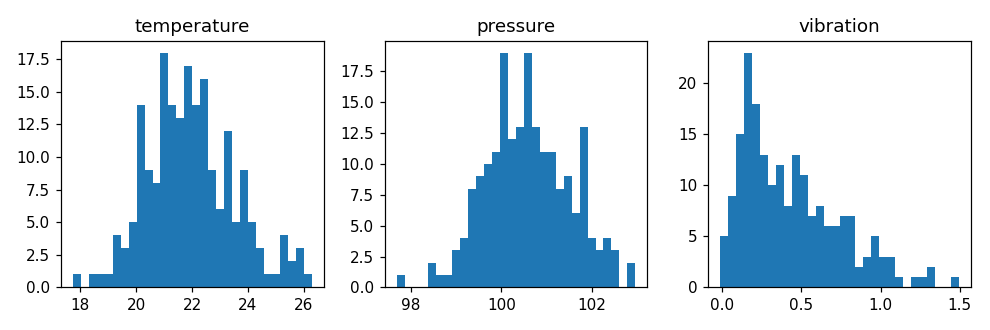
\includegraphics[width=0.9\textwidth]{../figures/histograms.png}
\caption{histograms.png}
\end{figure}
\begin{figure}[H]\centering
\includegraphics[width=0.9\textwidth]{../figures/time\_series.png}
\caption{time\_series.png}
\end{figure}
\begin{figure}[H]\centering
\includegraphics[width=0.9\textwidth]{../figures/forecast\_plot.png}
\caption{forecast\_plot.png}
\end{figure}
\section{Reproducibility}
All numbers in this report were computed locally by the deterministic Python engine; the LLM planned the methodology and interpreted the evidence. See \texttt{profile.json}, \texttt{gemini\_plan.json}, \texttt{manifest.json}. 
\end{document}
